\documentclass[11pt]{article}
\usepackage{geometry}                % See geometry.pdf to learn the layout options. There are lots.
\geometry{letterpaper}                   % ... or a4paper or a5paper or ... 
%\geometry{landscape}                % Activate for for rotated page geometry
%\usepackage[parfill]{parskip}    % Activate to begin paragraphs with an empty line rather than an indent
\usepackage{graphicx}
\usepackage{amssymb}
\usepackage{amsmath}
\usepackage{epstopdf}
\usepackage{hyperref}
\DeclareGraphicsRule{.tif}{png}{.png}{`convert #1 `dirname #1`/`basename #1 .tif`.png}


\graphicspath{
{/Users/Andy/Cruises_Research/Analysis/Andy_Pickering/eq08/figures/}
{/Users/Andy/Cruises_Research/Analysis/Andy_Pickering/eq08/figures/boot_eps_profiles_multprof/}
}

\title{Summary of $\chi$pod / Chameleon EQ08 Analysis}
\author{Andy Pickering}
%\date{}                                           % Activate to display a given date or no date



\begin{document}
\maketitle

\tableofcontents
\newpage


%~~~~~~~~~~~~~~~~~~~~~~~~~~~~~~~~~~~~~~~~
\section{Overview}
%~~~~~~~~~~~~~~~~~~~~~~~~~~~~~~~~~~~~~~~~

\begin{itemize}

\item This document is an attempt to provide an overview/summary of some analysis i've done with the EQ08 data. The motivation/goal for all this work is to show if /how well the CTD-$\chi$pod method works for estimating $\chi$,$\epsilon$, $K_T$, etc from fast temperature (thermistor) profiles. The idea is to deploy $\chi$pods on regular CTD casts on WOCE/CLIVAR cruises etc. to making mixing measurements.

\item Before dealing with all the issues with the CTD deployments (depth loops, entrained water, rosette-induced turbulence etc.), I wanted to verify that the method itself worked w/out these complications. 

\item The Chameleon microstructure profiler has both thermistor and shear probes, so this seemed like an ideal way to test the method. I would apply the $\chi$pod method to the chameleon thermistor data only ($\chi_{\chi},\epsilon_{\chi}$), and compare to the `true' results computed using the shear probes ($\chi$,$\epsilon$).


\end{itemize}




\clearpage
%~~~~~~~~~~~~~~~~~~~~~~~~~~~~~~~~~~~~~~~~
\section{Data and Processing}
%~~~~~~~~~~~~~~~~~~~~~~~~~~~~~~~~~~~~~~~~

\begin{itemize}

\item Data are from Chameleon profiles near the equator during the `EQ08' experiment.

\item $\chi$pod method is applied to thermistor data from Chameleon profiles in : \verb+ComputeChi_Chameleon_Eq08.m+

\item The noise floor of Chamleon $\epsilon$ was determined to be $log_{10}[\epsilon]=-8.5$. Values below this threshold were discarded. $\chi$pod values below this threshold were also discarded, in order to make a valid comparison. An upper limit of $log_{10}[\epsilon]=-5$ was also applied.

\item I re-processed the Chameleon data (\verb+run_eq08_AP.m+) using a fmax of 15hz for the $\chi$ calculations, based on looking at spectra and where they rolled off.

\item Data including surface convection was identified and excluded in the analysis. The mixed layer depth was identified using a criteria of $\sigma -\simga_{surface}=0.04$. This depth is shown in figures \ref{chi_overview} and \ref{eps_overview}. These depths were found w/ \verb+Identify_ML_eq08.m+

\item  The figures in this document are made w/ \verb+Make_Overview_Plots_eq08.m+.

\end{itemize}




\clearpage
%~~~~~~~~~~~~~~~~~~~~~~~~~~~~~~~~~~~~~~~~
\section{Results}
%~~~~~~~~~~~~~~~~~~~~~~~~~~~~~~~~~~~~~~~~


\subsection{Overview}

% misc_Appr14.m
\begin{figure}[htbp]
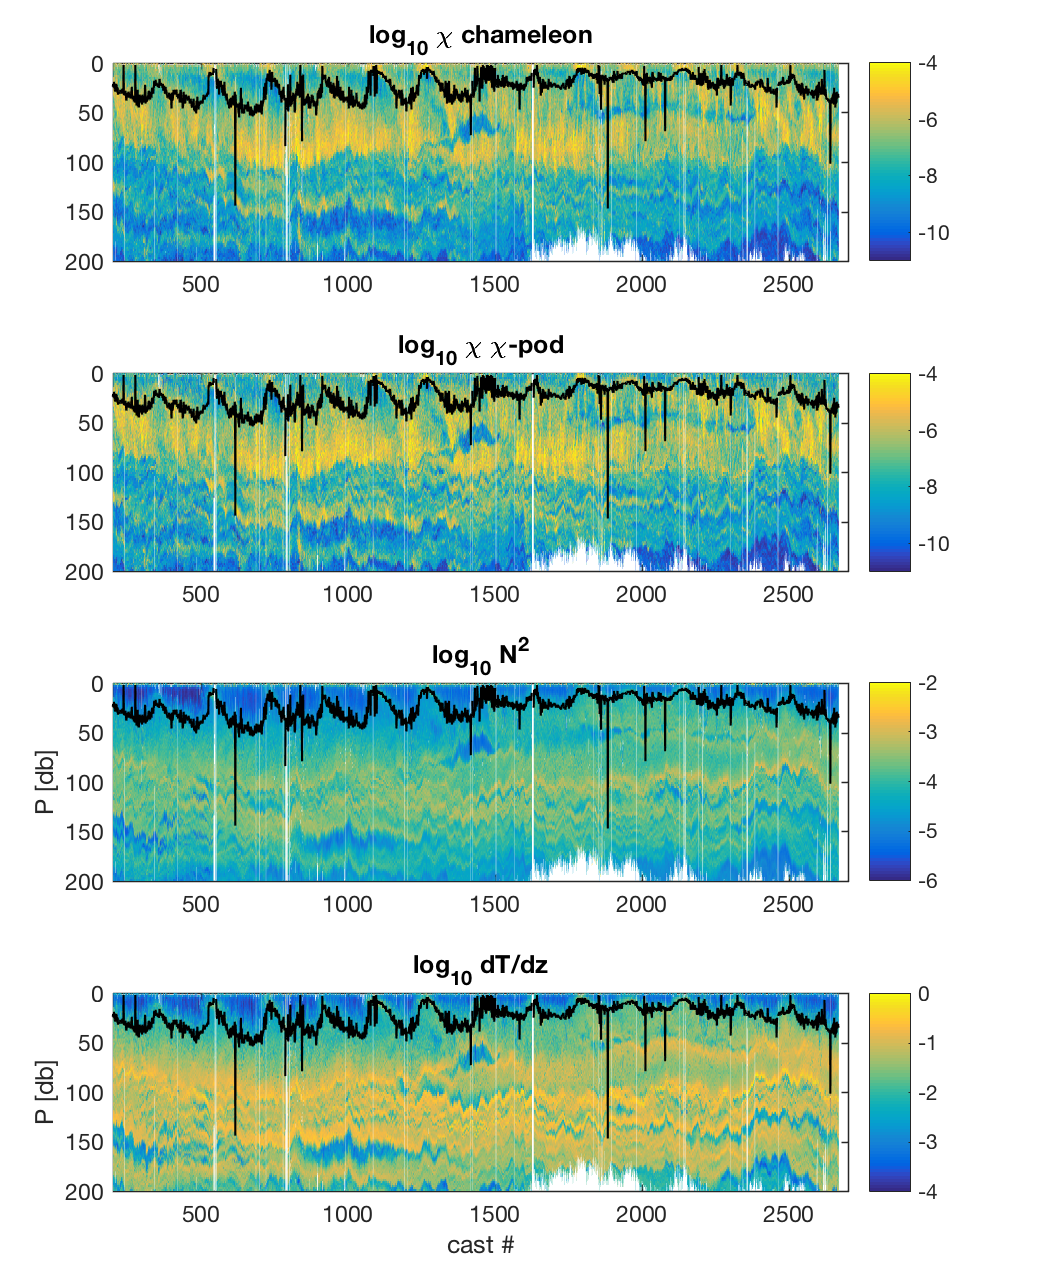
\includegraphics[scale=0.8]{eq08_Pcolor_BothChi_N2_Tz_screen_chi_1_zsm10m_fmax10Hz_respcorr0_fc_99hz_gamma20.png}
\caption{Comparison of $\chi$ from chameleon method and chi-pod method, for eq08 chameleon profiles. Date from each profile were averaged in 2m bins.  Black line shows shows convective regions excluded in further analysis.}
\label{chi_overview}
\end{figure}

\begin{figure}[htbp]
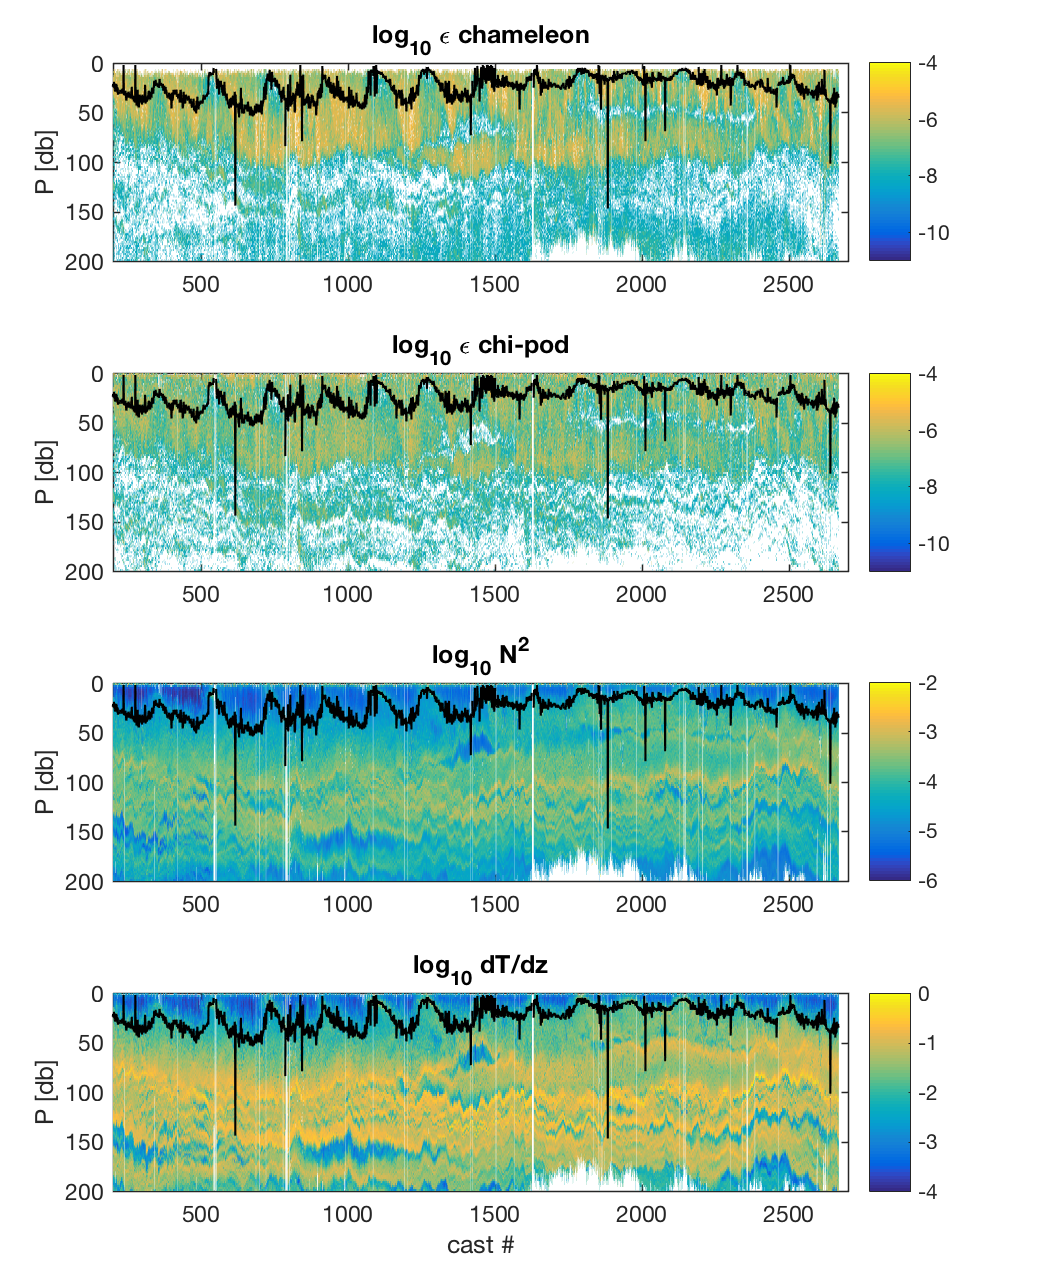
\includegraphics[scale=0.8]{eq08_Pcolor_BothEps_N2_Tz_screen_chi_1_zsm10m_fmax10Hz_respcorr0_fc_99hz_gamma20.png}
\caption{Comparison of $\epsilon$ from chameleon method and chi-pod method, for eq08 chameleon profiles. Each profile was averaged in 2m bins.  Values of $\epsilon_{\chi}$ and $\epsilon$ below chameleon noise floor ($log_{10}[\epsilon]=-8.5$) have been nan'd out. Black line shows shows convective regions excluded in further analysis.}
\label{eps_overview}
\end{figure}



\clearpage
%~~~~~~~~~~~~~~~~~~~~~~~~~~~~~~~~~~~~~~~~
\subsection{Comparing individual estimates of $\epsilon$}
%~~~~~~~~~~~~~~~~~~~~~~~~~~~~~~~~~~~~~~~~


\begin{itemize}

\item The $\chi$pod method tends to slightly over-estimate $\chi$, and underestimate $\epsilon$ (Figures \ref{chamVschi},\ref{epsrathist_eq08}). $\epsilon$ seems to be more under-estimated at higher values of $\epsilon$.

\item The bias in $\eposilon$ tends to be larger (more negative) at shallower depths (Figure \ref{2DvsP}).

\end{itemize}


%  plot of $\chi$pod vs cham for chi and eps
\begin{figure}[htbp]
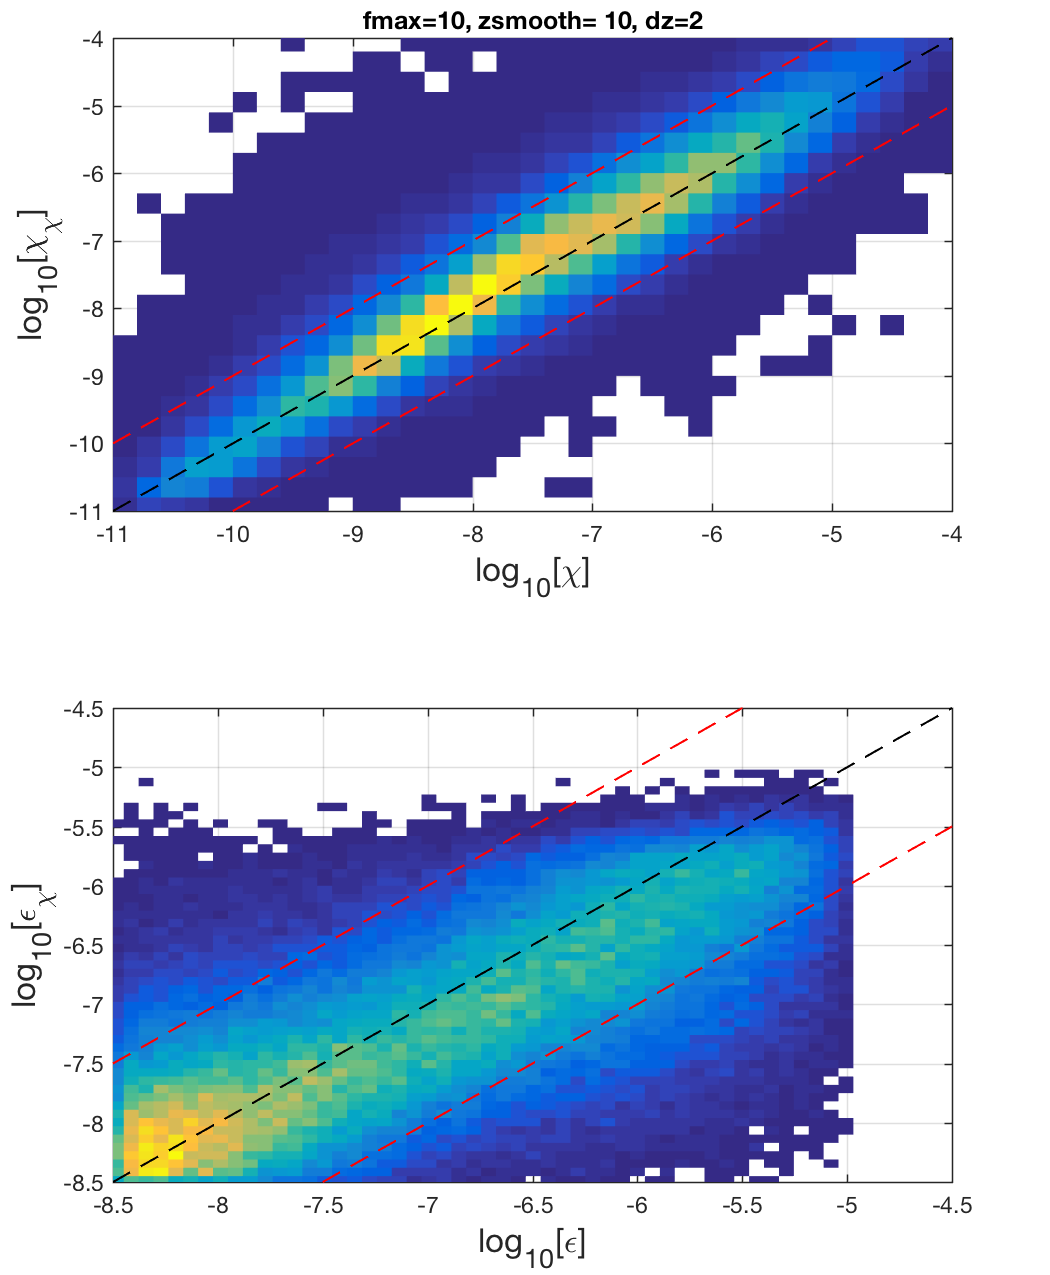
\includegraphics[scale=0.8]
{eq08_chamVschipod_screen_chi_1_Pmin_20_zsm10m_fmax10Hz_respcorr0_fc_99hz_gamma20.png}
\caption{Comparison of $\chi$ (top) and $\epsilon$ (lower) from chameleon method and chi-pod method, for eq08 chameleon profiles. Each profile was averaged in 2m bins.  Values of $\epsion$ below chameleon noise floor ($log_{10}[\epsilon]=-8.5$) have been nan'd out. Black line is 1:1, red lines are $+/-$ order of magnitude. }
\label{chamVschi}
\end{figure}


\begin{figure}[htbp]
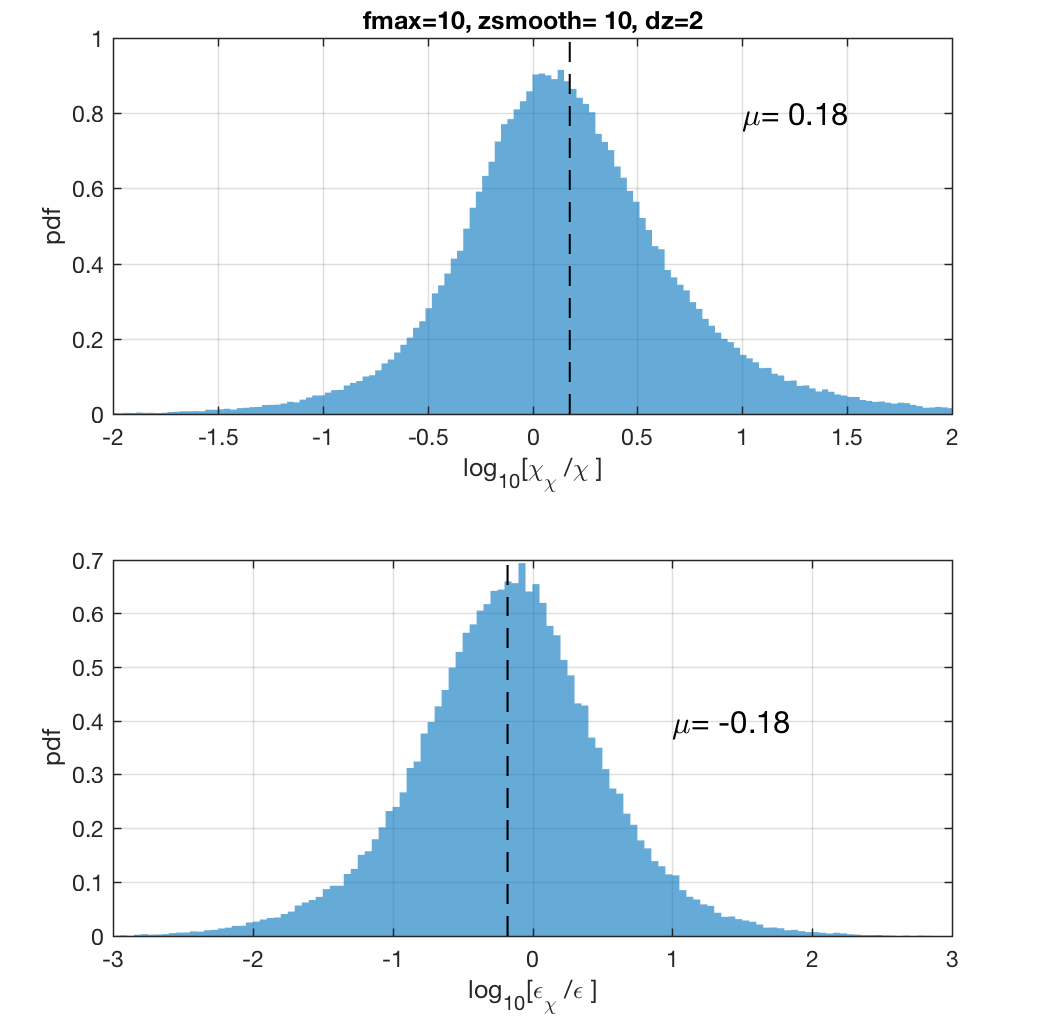
\includegraphics[scale=0.8]
{eq08_2mbinned_eps_ratios_screen_chi_1_screenml_1_zsm10m_fmax10Hz_respcorr0_fc_99hz_gamma20.png}
%{eq08_2mbinned_eps_ratios_screen_chi_1_zsm10m_fmax10Hz_respcorr0_fc_99hz_gamma20.png}
\caption{eq08: Histogram of the ratio of $\epsilon$ estimates from $\chi$pod method to the chameleon values. Estimates for each profile were averaged in 10m depth bins. Vertical line shows mean of $log_{10}[\epsilon_{\chi}/\epsilon]$.}
\label{epsrathist_eq08}
\end{figure}



\begin{figure}[htbp]
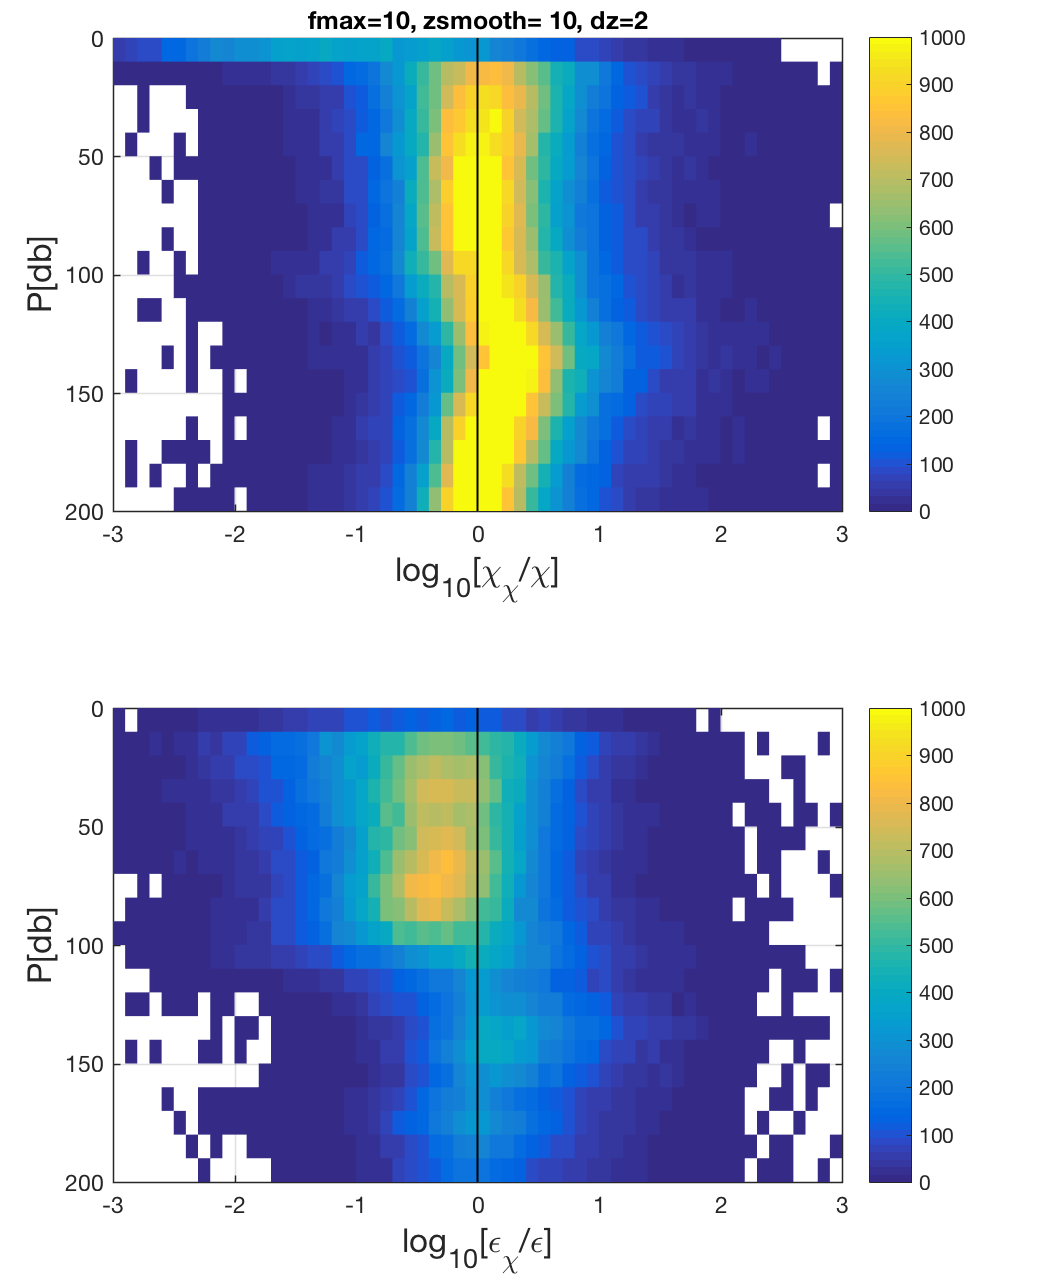
\includegraphics[scale=0.8]
{eq08_chi_eps_Vs_P_2Dhist_screen_chi_1_Pmin_0_zsm10m_fmax10Hz_respcorr0_fc_99hz_gamma20.png}
\caption{ 2D histograms of ratios $\chi_{\chi}/\chi$ and $\epsilon_{\chi}/\epsilon$ ratios vs depth.}
\label{2DvsP}
\end{figure}








\clearpage
%~~~~~~~~~~~~~~~~~~~~~~~~~~~~~~~~~~~~~~~~
\subsection{Normalized eps vs chi plots}
%~~~~~~~~~~~~~~~~~~~~~~~~~~~~~~~~~~~~~~~~

Assuming that
\begin{equation}
\gamma=\frac{N^2 \chi}{2\epsilon<T_z>^2}
\end{equation}
, plotting [$\chi/t_{z}^{2}$] vs [$\epsilon/N\^2$] should follow a straight line with slope equal to $2\gamma$. The Chameleon data from EQ08 tend to fall near $\gamma=0.1$ or slightly lower (Figure \ref{chiepsnorm}).


\begin{figure}[htbp]
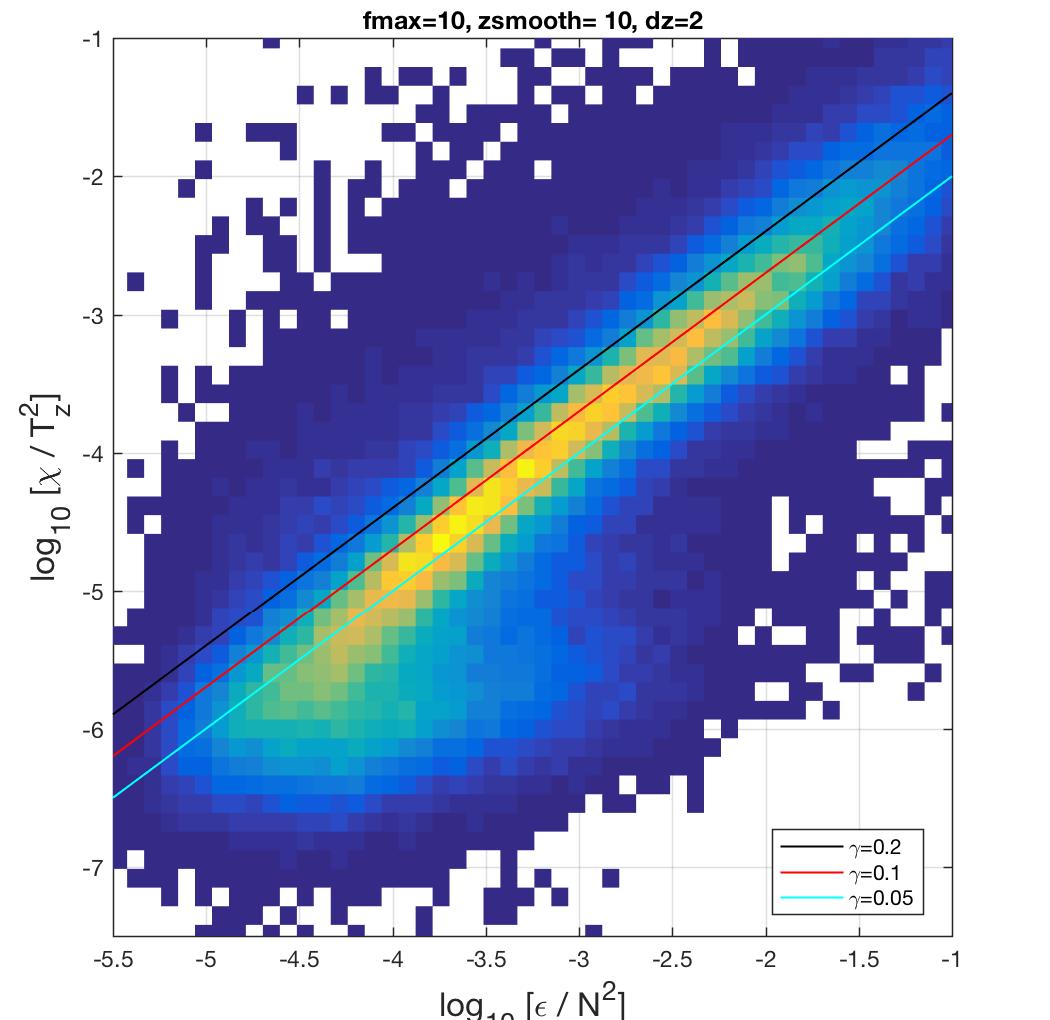
\includegraphics[scale=0.8]
{eq08_2mbinned_eps_vs_chi_normalized_zsm10m_fmax10Hz_respcorr0_fc_99hz_gamma20.png}
%{eq08_10mbinned_eps_vs_chi_normalized_zsm10m_fmax10Hz_respcorr0_fc_99hz_gamma20.png}
\caption{eq08: 10m binned  chameleon $\epsilon/N\^2$ vs $\chi/t_{z}^{2}$. Lines show different values of $\gamma$. Values of $\epsilon$ below noise floor ($log_{10}\epsilon<-8.5$) are discarded also.}
\label{chiepsnorm}
\end{figure}





\clearpage
%~~~~~~~~~~~~~~~~~~~~~~~~~~~~~~~~~~~~~~~~
\subsection{Averaging multiple profiles }
%~~~~~~~~~~~~~~~~~~~~~~~~~~~~~~~~~~~~~~~~


\begin{itemize}

\item 

\end{itemize}



\begin{figure}[htbp]
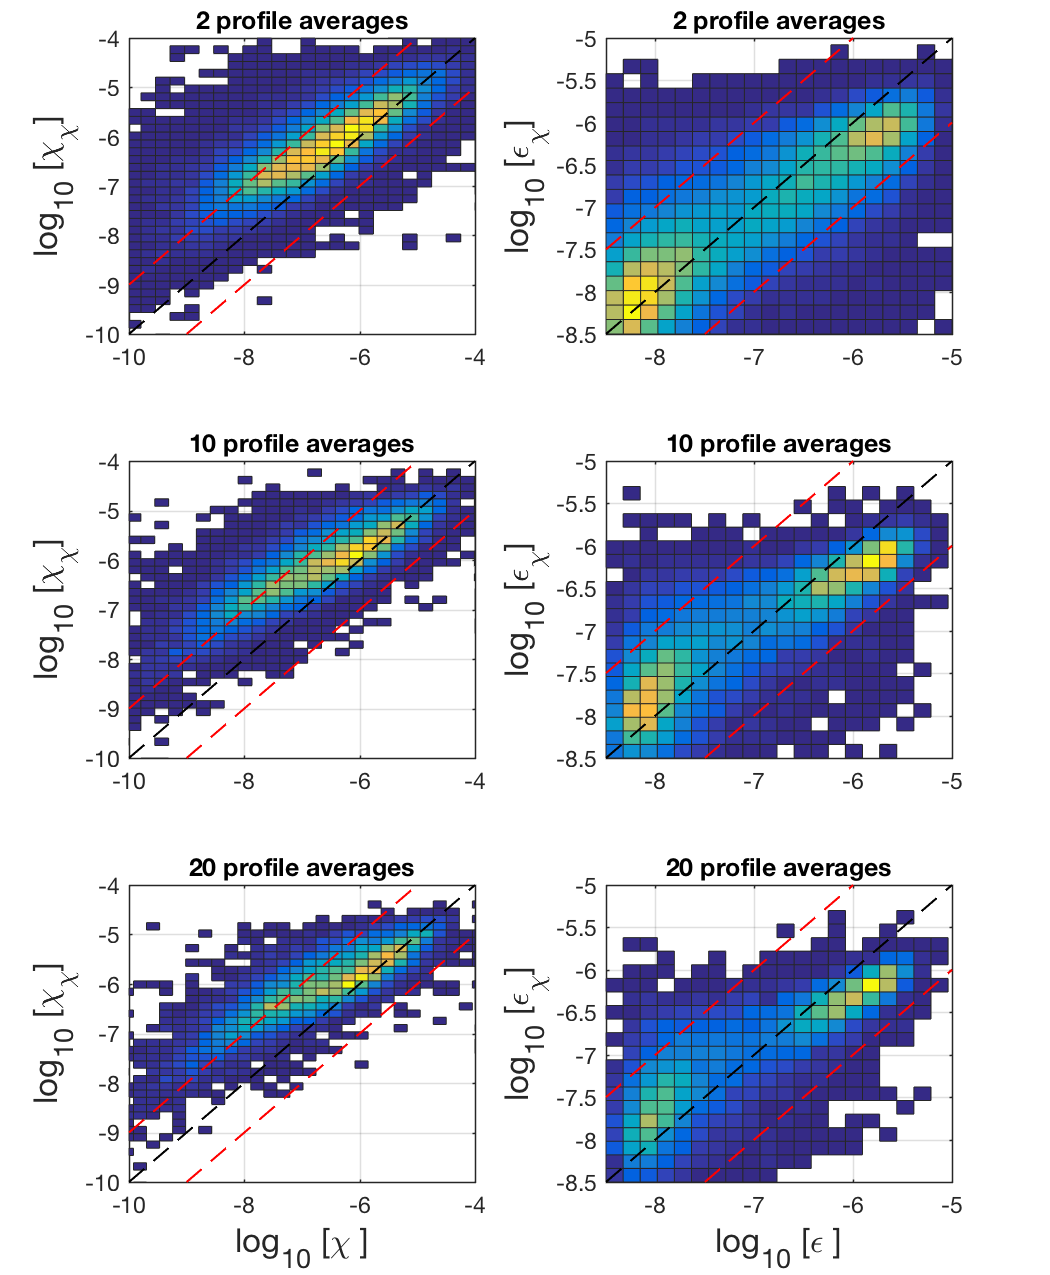
\includegraphics[scale=0.8]
{eq08_chiVscham_chiANDeps_diff_prof_avg_screen_chi_1_screen_ml_1_Pmin_20_dz_2_zsm10m_fmax10Hz_respcorr0_fc_99hz_gamma20.png}
\caption{2D Histograms of $\chi_{chi}$ vs $\chi$ (left) and $\epsilon_{\chi}$ vs $\epsilon$ (right) for different numbers of profiles averaged.}
\label{}
\end{figure}


\begin{figure}[htbp]
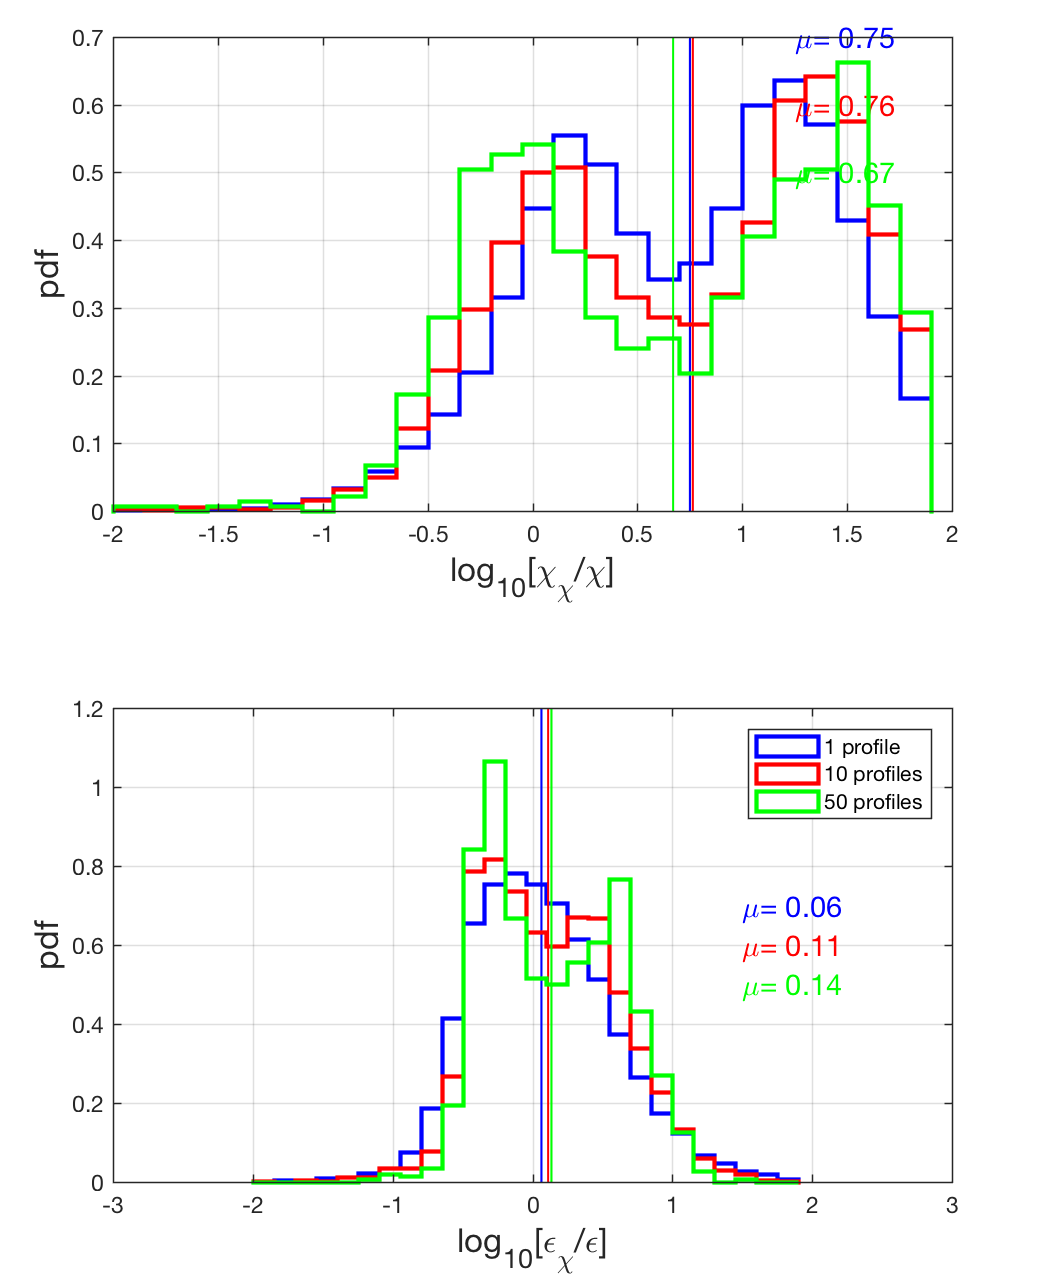
\includegraphics[scale=0.8]
{eq08_eps_ratio_hist_diff_prof_avg_Pmin_20zsm10m_fmax10Hz_respcorr0_fc_99hz_gamma20.png}
\caption{(log10) Ratio of $\epsilon_{\chi}/\epsilon$ for different numbers of profiles averaged. Consecutive chunks of N profiles were averaged, and then (normalized) histogram of the ratios was plotted. Vertical lines and numbers to right are mean of $log_{10}[\epsilon_{\chi}/\epsilon]$ for each distribution. }
\label{}
\end{figure}








\clearpage
%~~~~~~~~~~~~~~~~~~~~~~~~~~~~~~~~~~~~~~~~
\subsection{Averaging over different-sized depth bins}
%~~~~~~~~~~~~~~~~~~~~~~~~~~~~~~~~~~~~~~~~


I also looked at the effects of averaging each profile in different sized depth bins instead of averaging profiles.


\begin{itemize}

\item The bias in $\epsilon$ is decreased with averaging over larger depth intervals, although the bias in $\chi$ increases slightly (Figure \ref{hist_diffdz}).

\end{itemize}



\begin{figure}[htbp]
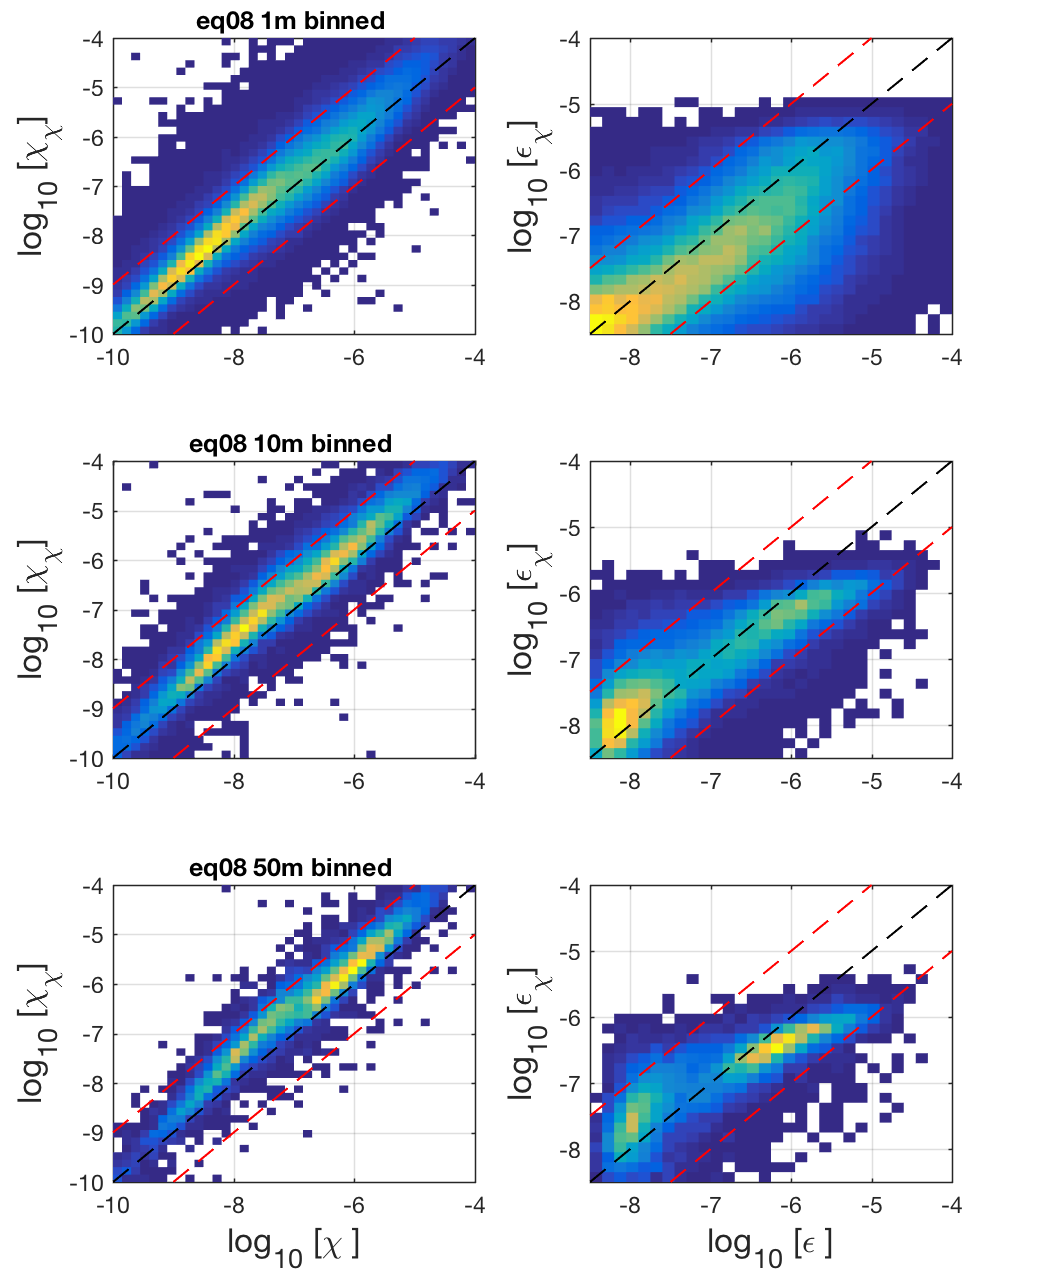
\includegraphics[scale=0.8]
{eq08_chiVscham_chiANDeps_diff_dz_screen_chi_1_Pmin_20_zsm10m_fmax10Hz_respcorr0_fc_99hz_gamma20.png}
\caption{2D Histograms of $\chi_{chi}$ vs $\chi$ (left) and $\epsilon_{\chi}$ vs $\epsilon$ (right) averaged over different size depth bins}
\label{2Dhist_diffdz}
\end{figure}



\begin{figure}[htbp]
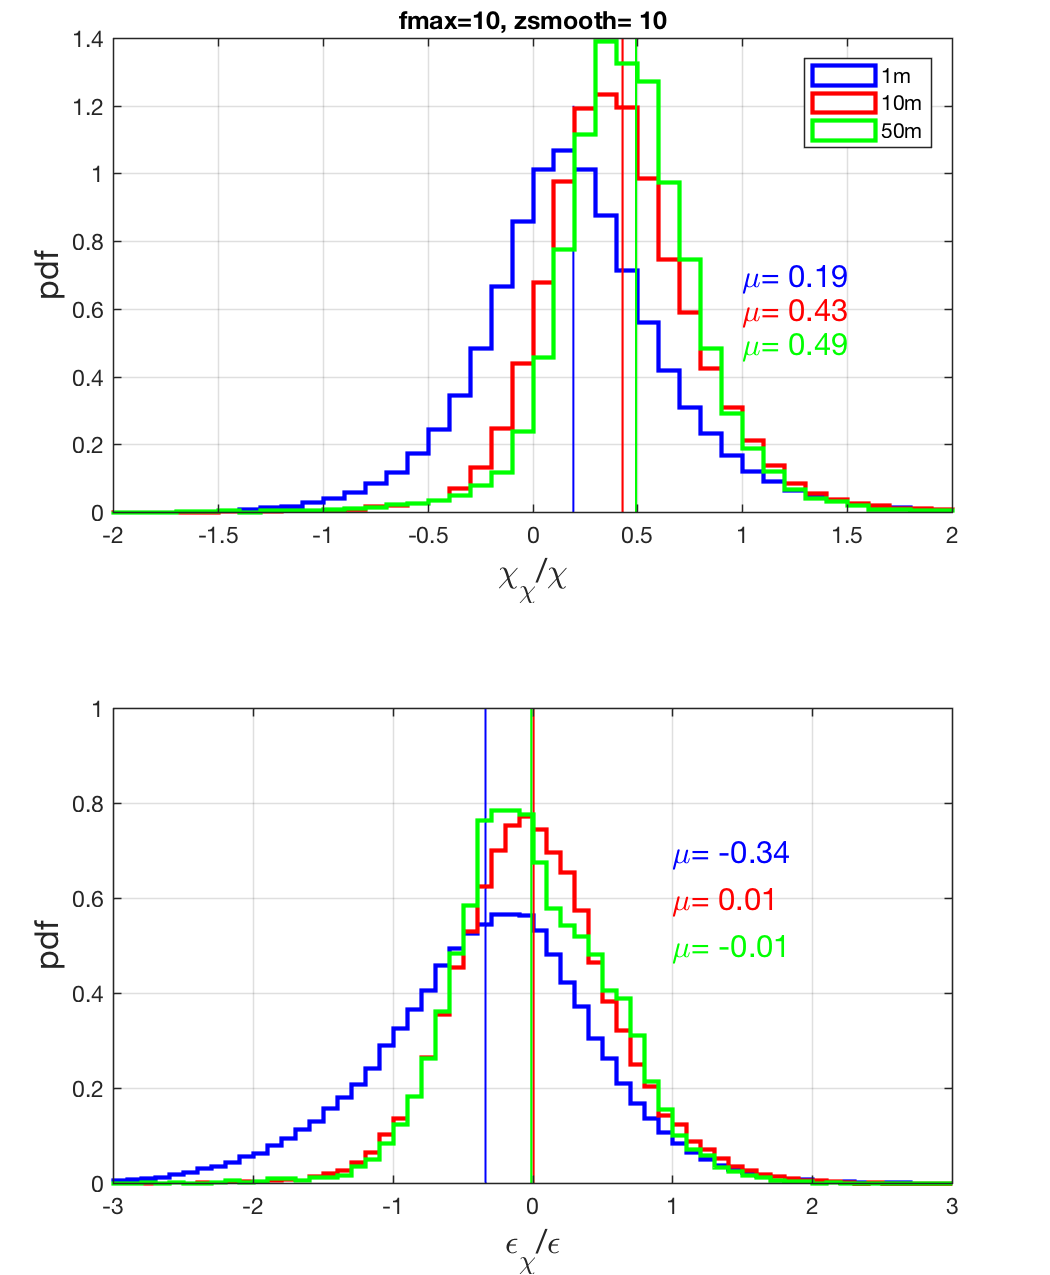
\includegraphics[scale=0.8]
{eq08_chiVscham_hist_diff_dz_screen_chi_1_Pmin_20_zsm10m_fmax10Hz_respcorr0_fc_99hz_gamma20.png}
\caption{Histogram of log10 of ratio $\epsilon_{\chi}/\epsilon$ for different amounts of vertical averaging. Vertical lines are mean of $log_{10}[\epsilon_{\chi}/\epsilon]$ for each distribution.}
\label{hist_diffdz}
\end{figure}







%\clearpage
%%~~~~~~~~~~~~~~~~~~~~~~~~~~~~~~~~~~~~~~~~
%\section{Summary}
%%~~~~~~~~~~~~~~~~~~~~~~~~~~~~~~~~~~~~~~~~
%
%\begin{itemize}
%
%\item Inidivudal (and 10m binned) $\chi$pod estimates of $\epsilon_{\chi}$ are biased low compared to Chameleon $\epsilon$.
%
%\item This appears to be because $\gamma$ computed from the Chameleon data is lower than the assumed 0.2
%
%%\item $\gamma$ computed from averaged data (across profiles) $N^2$, $T_z$, $\chi$, and $\epsilon$ is closer to 0.2
%
%\item Averaging $\epsilon$ over more profiles reduces the bias ?? (Figure \ref{}).
%
%\item Averaging $\epsilon$ over larger depth intervals reduces the bias (Figure \ref{}).
%
%
%\end{itemize}


\end{document}  


